\documentclass[11pt]{article}

% Font / typography
\usepackage[T1]{fontenc}
\usepackage{mathpazo}       % Palatino text + math (no external deps)
\usepackage[margin=1in]{geometry}

% Math
\usepackage{amsmath,amssymb,amsthm,mathtools}
\usepackage{enumitem}

% Figures / tables
\usepackage{graphicx}
\usepackage{booktabs}
\usepackage[section]{placeins}   % For \FloatBarrier

% Running header
\usepackage{fancyhdr}
\pagestyle{fancy}
\fancyhf{}
\fancyhead[R]{\footnotesize Muhamad Wakid \\ Independent researcher \\ ORCID: \href{https://orcid.org/0009-0008-6274-778X}{0009-0008-6274-778X}}
\renewcommand{\headrulewidth}{0.4pt}
\setlength{\headheight}{38pt}
\addtolength{\topmargin}{-14pt}

% Refs
\usepackage{xcolor}
\usepackage[colorlinks=true, linkcolor=blue!50!black, citecolor=blue!50!black,
            urlcolor=blue!50!black]{hyperref}

% Theorem environments
\newtheorem{theorem}{Theorem}
\newtheorem{proposition}[theorem]{Proposition}
\newtheorem{lemma}[theorem]{Lemma}
\newtheorem{corollary}[theorem]{Corollary}
\theoremstyle{remark}
\newtheorem{remark}[theorem]{Remark}

% Macros
\newcommand{\lcm}{\operatorname{lcm}}
\newcommand{\gcdop}{\operatorname{gcd}}
\newcommand{\PP}{\mathbb{P}}
\newcommand{\EE}{\mathbb{E}}
\newcommand{\one}{\mathbf{1}}
\newcommand{\PM}{\mathcal{P}_M}
\DeclareMathOperator{\Var}{Var}
\DeclareMathOperator{\Cov}{Cov}
\DeclareMathOperator{\Li}{Li}

\title{On the Expected Coprime Density of the\\[2pt]
Least Common Multiple of Random Integers}
\author{Muhamad Wakid}
\date{April 2026}

\begin{document}

\maketitle
\thispagestyle{fancy}

\begin{abstract}
Let $X_1, X_2, \ldots$ be independent and identically distributed random variables uniform on $\{2, 3, \ldots, M\}$, and let $L_k = \lcm(X_1, \ldots, X_k)$. We study the expected coprime density
\[
\rho_k(M) = \EE\!\left[\frac{\varphi(L_k)}{L_k}\right],
\]
where $\varphi$ is the Euler totient function. We establish an exact finite-sum identity for $\rho_k(M)$, written as a sum over subsets of primes $p \leq M$ and obtained by M\"obius inversion on the subset lattice. The identity implies $\rho_k(M) \to P_M := \prod_{p \leq M}(1 - 1/p)$ as $k \to \infty$ with $M$ fixed, with a sharp asymptotic equivalence $\rho_k(M) - P_M = P_M \Sigma_k(M)(1 + o(1))$ at geometric rate, where $\Sigma_k(M) = \sum_{p \leq M} q_p(M)^k/(p-1)$ and $q_p(M) = 1 - \lfloor M/p\rfloor/(M-1)$. In the joint regime $k = \lfloor cM \rfloor$, $M \to \infty$ (fixed $c > 0$), we prove the full asymptotic equivalence
\[
\ln M \cdot \frac{\rho_{\lfloor cM \rfloor}(M) - P_M}{P_M} \;\longrightarrow\; A(c) := \sum_{j \geq 1} e^{-cj} \ln\!\left(1 + \tfrac{1}{j}\right),
\]
strengthening the leading-order statement to an $o(1)$ remainder via a geometric-mean inequality for subset densities. Numerical computation to $M = 10^7$ across $15$ values of $c \in [0.05, 15]$ illustrates the finite-$M$ behaviour; linear extrapolation in $1/\ln M$ agrees with $A(c)$ to within approximately $0.5\%$ for $c \in [0.1, 5]$ and $1.5\%$ over the full tested range. The regime of fixed $M$ and growing $k$ is complementary to the fixed-$k$, $M \to \infty$ regime of the existing literature on random LCMs.
\end{abstract}

\noindent\textbf{Keywords:} Random LCM, Euler totient, Mertens product, Meissel--Mertens constant, probabilistic number theory, coprime density, M\"obius inversion, Rosser--Schoenfeld bounds.

\noindent\textbf{MSC 2020:} 11N37, 11K65, 11A25.

\section{Introduction}

The least common multiple of random integers is a classical object. Ces\`aro~\cite{Cesaro1885} showed that the expected LCM of two integers drawn uniformly from $\{1, \ldots, n\}$ is asymptotic to $n^2 \zeta(3)/\zeta(2)$ as $n \to \infty$. The subject has seen substantial recent development. Cilleruelo, Ru\'e, \v{S}arka, and Zumalac\'arregui~\cite{CilleruleoRueSarkaZumalacarregui2014} established almost-sure asymptotics for $\log \lcm$ of random subsets of $\{1, \ldots, n\}$; Fern\'andez and Fern\'andez~\cite{FernandezFernandez2021} surveyed divisibility properties of random tuples; Hilberdink and T\'oth~\cite{HilberdinkToth2016} obtained the average value of $\lcm$ of $k$ integers; Alsmeyer, Kabluchko, and Marynych~\cite{AlsmeyerKabluchkoMarynych2019} proved limit theorems for $\log \lcm$ of random sets; Bostan, Marynych, and Raschel~\cite{BostanMarynychRaschel2019} established distributional convergence of $f(L_n(k))/n^{r_k}$ for multiplicative functions $f$ of polynomial growth, where $L_n(k) = \lcm(X_1, \ldots, X_k)$ with $X_i$ uniform on $\{1, \ldots, n\}$ and $k$ fixed as $n \to \infty$; Buraczewski, Iksanov, and Marynych~\cite{BuraczewskiIksanovMarynych2022} established a central limit theorem for $\log \lcm$ of a uniformly sampled $m$-tuple; Iksanov, Marynych, and Raschel~\cite{IksanovMarynychRaschel2022} extended to hyperbolic regions; Kabluchko, Marynych, and Raschel~\cite{KabluchkoMarynychRaschel2023} to broader domains; and Sanna~\cite{Sanna2021} to $q$-analogues. A dissection of Mertens' prime product formula along a different axis (number of prime factors of summand integers) was given by Lichtman~\cite{Lichtman2021}.

These works share a common regime: the support size $n$ grows while the number of samples $k$ stays bounded. In this paper we study the opposite and complementary regime: the support $\{2, \ldots, M\}$ is fixed and the number of samples $k \to \infty$, plus the diagonal regime $k = \lfloor cM \rfloor$ with $M \to \infty$. The natural object of study in this regime is not the LCM itself --- which almost surely equals $\lcm(1, \ldots, M)$ for large $k$ --- but the arithmetic function
\[
\frac{\varphi(L_k)}{L_k} = \prod_{p \mid L_k}\!\left(1 - \frac{1}{p}\right),
\]
which measures the density of integers coprime to $L_k$. This quantity takes values in $(0, 1]$ and its large-$k$ behaviour is governed by exactly which primes $p \leq M$ appear as divisors of $L_k$. One expects the Mertens product as the limit, and this paper makes that expectation precise with explicit convergence rates. Second-order fluctuations --- the variance asymptotic and a central limit theorem for the centred log coprime density --- are developed in separate work in preparation.

\subsection{Main results}
Throughout, $M \geq 2$ is a fixed integer, $X_1, X_2, \ldots$ are i.i.d.\ uniform on $\{2, 3, \ldots, M\}$, $L_k = \lcm(X_1, \ldots, X_k)$, and $\rho_k(M) = \EE[\varphi(L_k)/L_k]$. Write $\PM = \{p : p \leq M\}$, $m_p = \lfloor M/p \rfloor$, and $q_p(M) = 1 - m_p/(M-1)$, the probability that a single uniform draw from $\{2, \ldots, M\}$ is not a multiple of $p$. For $T \subseteq \PM$, let
\[
\beta_T(M) = \frac{1}{M-1}\,\Bigl|\bigl\{n \in \{2, \ldots, M\} : \gcdop\bigl(n, \textstyle\prod_{p \in T} p\bigr) = 1\bigr\}\Bigr|.
\]
The Mertens product up to $M$ is $P_M := \prod_{p \leq M}(1 - 1/p)$.

\begin{theorem}[Exact identity]\label{thm:identity}
For every $M \geq 2$ and every $k \geq 1$,
\begin{equation}\label{eq:identity}
\rho_k(M) = P_M \sum_{T \subseteq \PM} \beta_T(M)^k \prod_{p \in T} \frac{1}{p-1}.
\end{equation}
\end{theorem}

\begin{theorem}[Limit and rate]\label{thm:limit-rate}
Let $\Sigma_k(M) := \sum_{p \leq M} q_p(M)^k/(p-1)$ and $\Lambda(M) := \sum_{p \leq M} 1/(p-1)$. For every fixed $M \geq 2$, $\lim_{k \to \infty} \rho_k(M) = P_M$, and
\begin{equation}\label{eq:decomp}
\frac{\rho_k(M) - P_M}{P_M} = \Sigma_k(M) + R_k(M),
\end{equation}
where $R_k(M) \geq 0$ satisfies
\begin{equation}\label{eq:Rk-bound}
R_k(M) \leq \frac{1}{2}\,\Sigma_{k/2}(M)^2 \, e^{\Lambda(M)}.
\end{equation}
In particular $R_k(M) \to 0$ and $\Sigma_k(M) \to 0$ as $k \to \infty$, establishing $\rho_k(M) \to P_M$.
\end{theorem}

\begin{remark}\label{rem:sharp-fixed-M}
The bound~\eqref{eq:Rk-bound} establishes $R_k(M) \to 0$ at exponential rate at fixed $M$, but as an asymptotic equivalence it gives only $R_k(M) = O(\Sigma_{k/2}(M)^2)$, which at fixed $M$ is $O(1) \cdot \Sigma_k(M)$ rather than $o(1)\cdot \Sigma_k(M)$. The sharper conclusion does \emph{not} follow from~\eqref{eq:Rk-bound} alone; in particular it would follow from the na\"ive independence bound $\beta_T(M) \leq \prod_{p \in T} q_p(M)$, which however fails in a nontrivial set of small-$M$ examples. For instance, at $M = 17$ and $T = \{3, 5\}$ one has $\beta_T = 9/16$ while $q_3 q_5 = 143/256$, with excess $1/256 \approx 3.9 \times 10^{-3}$; the worst violation we observed over $M \leq 50$ is $1/90 \approx 1.1 \times 10^{-2}$, at $M = 31$, $T = \{2, 3, 7\}$. Theorem~\ref{thm:sharp-fixed-M} below obtains the sharp equivalence by a different, simpler route.
\end{remark}

\begin{theorem}[Sharp form at fixed $M$]\label{thm:sharp-fixed-M}
For every fixed $M \geq 3$, as $k \to \infty$,
\begin{equation}\label{eq:sharp-fixed-M}
\frac{R_k(M)}{\Sigma_k(M)} = O\!\left(\left(\frac{q^{**}(M)}{q^{*}(M)}\right)^{\!k}\right),
\end{equation}
where $q^{*}(M) := \max_{p \leq M} q_p(M)$ and $q^{**}(M) := \max_{T \subseteq \PM,\, |T| \geq 2}\, \beta_T(M)$ satisfy $q^{**}(M) < q^{*}(M)$. In particular $R_k(M) = o(\Sigma_k(M))$ as $k \to \infty$, and
\[
\rho_k(M) - P_M = P_M\, \Sigma_k(M)\,\bigl(1 + o(1)\bigr) \qquad (k \to \infty,\; M \text{ fixed}).
\]
Moreover, for $M \geq 11$, elementary enumeration shows there are at least two primes in $(M/2, M]$ (a consequence of Ramanujan's strengthening of Bertrand's postulate~\cite{Ramanujan1919}), giving $q^{**}(M) = (M-3)/(M-1)$ and $q^{*}(M) = (M-2)/(M-1)$, so that $q^{**}(M)/q^{*}(M) = (M-3)/(M-2)$ and the rate of convergence is explicit.
\end{theorem}

\begin{theorem}[Joint scaling, sharp form]\label{thm:joint-sharp}
For each fixed $c > 0$,
\begin{equation}\label{eq:sigma-limit}
\lim_{M \to \infty} \ln M \cdot \Sigma_{\lfloor cM \rfloor}(M) = A(c),
\end{equation}
where
\begin{equation}\label{eq:A-def}
A(c) := \sum_{j \geq 1} e^{-cj} \ln\!\left(1 + \frac{1}{j}\right),
\end{equation}
and moreover
\begin{equation}\label{eq:sharp}
\lim_{M \to \infty} \ln M \cdot \frac{\rho_{\lfloor cM \rfloor}(M) - P_M}{P_M} = A(c).
\end{equation}
\end{theorem}

The leading-order assertion~\eqref{eq:sigma-limit} is established via Mertens' second theorem, Rosser--Schoenfeld bounds, and dominated convergence. The sharp form~\eqref{eq:sharp} requires a genuinely new ingredient: a geometric-mean bound for subset densities (Lemma~\ref{lem:geom-mean} below) that controls the multi-prime correction $R_k$ uniformly.

\begin{proposition}[Asymptotic behaviour of $A$]\label{prop:A-asymptotics}
The function $A \colon (0, \infty) \to (0, \infty)$ is smooth, strictly decreasing, and strictly convex. Moreover:
\begin{enumerate}[label=(\roman*), leftmargin=2em]
\item As $c \to 0^+$,
\[
A(c) = -\ln c - \gamma - \frac{c \ln c}{2} + O(c),
\]
where $\gamma$ is the Euler--Mascheroni constant.
\item As $c \to \infty$,
\[
A(c) = e^{-c} \ln 2 + e^{-2c} \ln \tfrac{3}{2} + e^{-3c}\ln\tfrac{4}{3} + O(e^{-4c}).
\]
\end{enumerate}
\end{proposition}

\subsection{Organisation}
Section~\ref{sec:prelim} fixes notation and records elementary lemmas, including the new geometric-mean bound Lemma~\ref{lem:geom-mean}. Sections~\ref{sec:thm1},~\ref{sec:thm2},~\ref{sec:thm-sharp-fixed-M}, and~\ref{sec:thm4} prove Theorems~\ref{thm:identity},~\ref{thm:limit-rate},~\ref{thm:sharp-fixed-M}, and~\ref{thm:joint-sharp} respectively. Section~\ref{sec:numerics} presents numerical evidence. Section~\ref{sec:discussion} discusses the fluctuations problem and other extensions. Section~\ref{sec:conclusion} concludes.

\section{Preliminaries}\label{sec:prelim}

Notation is standard: $\varphi$ is Euler's totient, $p$ ranges over primes, $\mathcal{P}(n) = \{p : p \mid n\}$, and $\PM = \{p : p \leq M\}$. We use $\ln$ (natural logarithm) throughout; the Mertens product is $P_M = \prod_{p \leq M}(1 - 1/p)$.

For $p \in \PM$, every multiple of $p$ in $\{1, \ldots, M\}$ also lies in $\{2, \ldots, M\}$ since $p \geq 2$, so $m_p = \lfloor M/p \rfloor$ equals the number of multiples of $p$ in the sampling space. For $T \subseteq \PM$, let $A_T(M) = \{n \in \{2, \ldots, M\} : \gcdop(n, \prod_{p \in T} p) = 1\}$, so $\beta_T(M) = |A_T(M)|/(M-1)$, $\beta_\emptyset(M) = 1$, and $\beta_{\{p\}}(M) = q_p(M)$.

\begin{lemma}\label{lem:betaT-power}
For any $T \subseteq \PM$,
\[
\PP\bigl(\forall i \leq k,\; X_i \in A_T(M)\bigr) = \beta_T(M)^k,
\]
equivalently, $\PP(\text{no prime in $T$ divides $L_k$}) = \beta_T(M)^k$.
\end{lemma}
\begin{proof}
Immediate from independence of $X_1, \ldots, X_k$ and the fact that $p \mid L_k$ iff $p \mid X_i$ for some $i$.
\end{proof}

\begin{lemma}\label{lem:single-prime}
For any $\emptyset \neq T \subseteq \PM$ and any $p_0 \in T$, $\beta_T(M) \leq q_{p_0}(M)$.
\end{lemma}
\begin{proof}
$A_T(M) \subseteq \{n \in \{2, \ldots, M\} : p_0 \nmid n\}$.
\end{proof}

\begin{lemma}[Two-prime bound for $|T| \geq 2$]\label{lem:two-prime}
Let $T \subseteq \PM$ with $|T| \geq 2$, and let $p_0, p_1$ be any two distinct elements of $T$. Then for every $k \geq 1$,
\[
\beta_T(M)^k \leq q_{p_0}(M)^{k/2}\, q_{p_1}(M)^{k/2}.
\]
\end{lemma}
\begin{proof}
By Lemma~\ref{lem:single-prime} applied to each of $p_0, p_1$, $\beta_T(M)^{k/2} \leq q_{p_0}(M)^{k/2}$ and $\beta_T(M)^{k/2} \leq q_{p_1}(M)^{k/2}$. Multiply.
\end{proof}

\begin{lemma}[Geometric-mean bound for $|T| \geq 1$]\label{lem:geom-mean}
Let $T \subseteq \PM$ with $|T| = r \geq 1$. For every real $k > 0$,
\begin{equation}\label{eq:geom-mean}
\beta_T(M)^k \leq \prod_{p \in T} q_p(M)^{k/r}.
\end{equation}
\end{lemma}
\begin{proof}
By Lemma~\ref{lem:single-prime}, $\beta_T(M) \leq q_p(M)$ for every $p \in T$. Multiplying these $r$ inequalities gives $\beta_T(M)^r \leq \prod_{p \in T} q_p(M)$, and taking both sides to the positive real power $k/r$ preserves the inequality since both sides lie in $(0, 1]$. Rewriting the right-hand side as $\prod_{p \in T} q_p(M)^{k/r}$ gives~\eqref{eq:geom-mean}.
\end{proof}

\begin{remark}\label{rem:why-geom-mean}
Lemma~\ref{lem:geom-mean} is the key new ingredient for the sharp form~\eqref{eq:sharp} of Theorem~\ref{thm:joint-sharp}. Lemma~\ref{lem:two-prime} suffices for~\eqref{eq:sigma-limit} at leading order but forces an $O(1)$ remainder via the factor $e^{\Lambda(M)}$ in~\eqref{eq:Rk-bound}. The stronger bound~\eqref{eq:geom-mean} permits a stratification of the multi-prime sum by $|T|$ that avoids the wasteful $e^{\Lambda(M)}$ factor, at the cost of using $\Sigma_{k/r}$ rather than $\Sigma_{k/2}$ for terms with $|T| = r \geq 3$.
\end{remark}

\begin{remark}\label{rem:betaT-violation}
The na\"ive bound $\beta_T(M) \leq \prod_{p \in T} q_p(M)$, which would be valid under independence, fails in general: for instance at $(M, T) = (17, \{3, 5\})$ direct enumeration gives $\beta_T = 9/16 \approx 0.5625$ while $q_3 q_5 = (11/16)(13/16) = 143/256 \approx 0.5586$. The failure arises because the events $\{p \mid X\}$ for different primes $p$ are not independent on the finite sample space $\{2, \ldots, M\}$. Lemma~\ref{lem:geom-mean} provides the alternative bound actually needed for the proof of Theorem~\ref{thm:joint-sharp}.
\end{remark}

\section{Proof of Theorem~\ref{thm:identity}}\label{sec:thm1}

For each $S \subseteq \PM$, let $E_S = \{\mathcal{P}(L_k) = \PM \setminus S\}$ be the event that the set of primes dividing $L_k$ is exactly $\PM \setminus S$. On $E_S$,
\begin{equation}\label{eq:phi-over-L-on-ES}
\frac{\varphi(L_k)}{L_k} = \prod_{p \in \PM \setminus S}\!\left(1 - \frac{1}{p}\right) = \frac{P_M}{\prod_{p \in S}(1 - 1/p)} = P_M \prod_{p \in S} \frac{p}{p-1}.
\end{equation}
The events $\{E_S\}_{S \subseteq \PM}$ partition the sample space (primes $> M$ never divide any $X_i$), so
\begin{equation}\label{eq:rho-by-ES}
\rho_k(M) = P_M \sum_{S \subseteq \PM} \PP(E_S) \prod_{p \in S} \frac{p}{p-1}.
\end{equation}
Now $E_S = \{\text{no prime in $S$ divides $L_k$}\} \cap \{\text{every prime in $\PM \setminus S$ divides $L_k$}\}$, so by M\"obius inversion on the subset lattice,
\begin{equation}\label{eq:ES-by-mobius}
\PP(E_S) = \sum_{T \colon S \subseteq T \subseteq \PM} (-1)^{|T|-|S|}\, \PP(\text{no prime in $T$ divides $L_k$}) = \sum_{T \supseteq S} (-1)^{|T|-|S|}\, \beta_T(M)^k,
\end{equation}
by Lemma~\ref{lem:betaT-power}. Substituting~\eqref{eq:ES-by-mobius} into~\eqref{eq:rho-by-ES} and swapping the order of summation,
\[
\rho_k(M) = P_M \sum_{T \subseteq \PM} \beta_T(M)^k \sum_{S \subseteq T} (-1)^{|T|-|S|} \prod_{p \in S} \frac{p}{p-1}.
\]
The inner sum factors over primes in $T$:
\[
\sum_{S \subseteq T} (-1)^{|T|-|S|} \prod_{p \in S} \frac{p}{p-1} = \prod_{p \in T}\!\left(\frac{p}{p-1} - 1\right) = \prod_{p \in T} \frac{1}{p-1}. \qedhere
\]

\section{Proof of Theorem~\ref{thm:limit-rate}}\label{sec:thm2}

Starting from~\eqref{eq:identity} and isolating $T = \emptyset$ (contribution $P_M$),
\[
\frac{\rho_k(M) - P_M}{P_M} = \sum_{T \subseteq \PM,\; T \neq \emptyset} \beta_T(M)^k \prod_{p \in T} \frac{1}{p-1}.
\]
The $|T| = 1$ contributions sum to $\Sigma_k(M)$. Denote the sum of the $|T| \geq 2$ contributions by $R_k(M)$.

To bound $R_k(M)$, group each $T$ with $|T| \geq 2$ by its two smallest primes. For each pair $\{p_0, p_1\}$ with $p_0 < p_1 \in \PM$, let $\mathcal{T}(p_0, p_1) = \{T \subseteq \PM : \min T = p_0,\; \text{second-min}\, T = p_1\}$. Then every $T$ with $|T| \geq 2$ lies in exactly one such class, and $T \in \mathcal{T}(p_0, p_1)$ iff $T = \{p_0, p_1\} \cup U$ for some $U \subseteq \PM \cap (p_1, \infty)$. By Lemma~\ref{lem:two-prime},
\begin{align*}
R_k(M) &= \sum_{p_0 < p_1 \in \PM} \sum_{T \in \mathcal{T}(p_0, p_1)} \beta_T(M)^k \prod_{p \in T} \frac{1}{p-1} \\
&\leq \sum_{p_0 < p_1} \frac{q_{p_0}(M)^{k/2}}{p_0 - 1}\cdot \frac{q_{p_1}(M)^{k/2}}{p_1 - 1} \sum_{U \subseteq \PM \cap (p_1, \infty)} \prod_{p \in U} \frac{1}{p-1} \\
&\leq \sum_{p_0 < p_1} \frac{q_{p_0}(M)^{k/2}}{p_0 - 1}\cdot \frac{q_{p_1}(M)^{k/2}}{p_1 - 1} \cdot e^{\Lambda(M)},
\end{align*}
using $\sum_U \prod_{p \in U} 1/(p-1) = \prod_{p \leq M}(1 + 1/(p-1)) \leq e^{\Lambda(M)}$. The inequality $\sum_{p_0 < p_1} a_{p_0} a_{p_1} \leq \tfrac12(\sum_p a_p)^2$ with $a_p = q_p(M)^{k/2}/(p-1)$ gives~\eqref{eq:Rk-bound}.

For the limit: each $q_p(M) < 1$ and $\PM$ is finite, so $\Sigma_k(M) \to 0$ as $k \to \infty$; and $\Sigma_{k/2}(M) \to 0$ similarly, so $R_k(M) \to 0$ by~\eqref{eq:Rk-bound}. Hence $(\rho_k(M) - P_M)/P_M \to 0$, i.e.\ $\rho_k(M) \to P_M$. \qed

\section{Proof of Theorem~\ref{thm:sharp-fixed-M}}\label{sec:thm-sharp-fixed-M}

Recall $R_k(M) = \sum_{T \subseteq \PM,\, |T| \geq 2}\beta_T(M)^k \prod_{p \in T}\frac{1}{p-1}$.

\emph{Step 1: $q^{**}(M) < q^{*}(M)$ for $M \geq 3$.} Fix any $T \subseteq \PM$ with $|T| \geq 2$ and pick distinct $p_0, p_1 \in T$. By Lemma~\ref{lem:single-prime}, $\beta_T(M) \leq q_{p_0}(M) \leq q^*(M)$. We show the first inequality is strict, which gives $\beta_T < q^*$.

Strict inclusion $A_T(M) \subsetneq A_{\{p_0\}}(M)$ holds because $p_1$ itself, viewed as an integer in $\{2, \ldots, M\}$, belongs to $A_{\{p_0\}}(M) \setminus A_T(M)$: indeed $p_1$ is coprime to $p_0$ (distinct primes) so $p_1 \in A_{\{p_0\}}(M)$, but $p_1$ is divisible by $p_1 \in T$ so $p_1 \notin A_T(M)$. Hence $|A_T| < |A_{\{p_0\}}|$, i.e.\ $\beta_T < q_{p_0}$. Since this holds for every $T$ with $|T| \geq 2$, $q^{**}(M) < q^*(M)$.

\emph{Step 2: bound on $R_k$.} For every $T$ with $|T| \geq 2$, $\beta_T \leq q^{**}$, so
\[
R_k(M) = \sum_{|T| \geq 2}\beta_T^k \prod_{p \in T}\frac{1}{p-1} \leq (q^{**})^k \sum_{|T| \geq 2}\prod_{p \in T}\frac{1}{p-1}.
\]
The last sum is at most $\prod_{p \leq M}(1 + 1/(p-1)) = \prod_{p \leq M}p/(p-1) = 1/P_M \leq e^{\Lambda(M)}$ (Mertens). Hence
\begin{equation}\label{eq:Rk-qstarstar}
R_k(M) \leq (q^{**}(M))^k \cdot e^{\Lambda(M)}.
\end{equation}

\emph{Step 3: lower bound on $\Sigma_k$.} Let $p^*$ be any prime with $q_{p^*}(M) = q^*(M)$. Then
\begin{equation}\label{eq:Sigma-qstar}
\Sigma_k(M) \geq \frac{(q^*(M))^k}{p^* - 1} \geq \frac{(q^*(M))^k}{M-1}.
\end{equation}

\emph{Step 4: combining.} Dividing~\eqref{eq:Rk-qstarstar} by~\eqref{eq:Sigma-qstar},
\[
\frac{R_k(M)}{\Sigma_k(M)} \leq (M-1)\, e^{\Lambda(M)}\left(\frac{q^{**}(M)}{q^*(M)}\right)^{\!k}.
\]
Since $q^{**} < q^*$ (Step~1), the right-hand side tends to $0$ geometrically in $k$, establishing~\eqref{eq:sharp-fixed-M}.

\emph{Step 5: explicit rate for $M \geq 11$.} For $M \geq 11$, by Ramanujan's strengthening of Bertrand's postulate~\cite{Ramanujan1919} there are at least two primes in $(M/2, M]$; call them $p_1, p_2$. Both have $m_p = 1$, so $q_{p_i} = (M-2)/(M-1) = q^*$. For $T = \{p_1, p_2\}$, $p_1 p_2 > (M/2)^2 \geq M$ (for $M \geq 4$), so $\lfloor M/(p_1 p_2)\rfloor = 0$ and $\beta_T = (M - 2 - 2 + 0 - 1)/(M-1) = (M-3)/(M-1)$ by direct inclusion-exclusion. To see this is the maximum: any other $T$ with $|T| \geq 2$ satisfies either (i)~$T \subseteq \PM \cap (M/2, M]$, in which case $\beta_T = (M - |T| - 1)/(M-1) \leq (M-3)/(M-1)$ since $|T| \geq 2$; or (ii)~$T$ contains some $p$ with $m_p \geq 2$, in which case $\beta_T \leq q_p \leq (M-3)/(M-1)$ (since $q_p = 1 - m_p/(M-1) \leq (M-3)/(M-1)$). Hence $q^{**}(M) = (M-3)/(M-1)$.
\qed

\section{Proof of Theorem~\ref{thm:joint-sharp}}\label{sec:thm4}

We prove~\eqref{eq:sigma-limit} first and then derive~\eqref{eq:sharp} from Lemma~\ref{lem:geom-mean}.

\subsection{Proof of~\eqref{eq:sigma-limit}: leading-order convergence of $\Sigma$}\label{sec:thm4-leading}

Partition primes by $m_p$-value. A prime $p$ satisfies $m_p = j$ iff $p \in (M/(j+1), M/j]$. For such $p$, $q_p(M) = 1 - j/(M-1)$. Write
\[
S_j(M) := \sum_{p \in \PM \colon m_p = j} \frac{1}{p-1},
\]
so $\Sigma_{\lfloor cM \rfloor}(M) = \sum_{j \geq 1}(1 - j/(M-1))^{\lfloor cM \rfloor}\, S_j(M)$.

\emph{Pointwise limit.} For each fixed $j \geq 1$, using $\ln(1 - x) = -x + O(x^2)$ as $x \to 0$,
\[
\bigl(1 - j/(M-1)\bigr)^{\lfloor cM \rfloor} = \exp\bigl(\lfloor cM \rfloor(-j/(M-1) + O(1/M^2))\bigr) \longrightarrow e^{-cj}.
\]
By the prime number theorem with a classical de la Vall\'ee Poussin error term~\cite[Ch.~I.3]{Tenenbaum2015}, partial summation yields the sharpened form of Mertens' second theorem
\[
\sum_{p \leq x} \frac{1}{p} = \ln \ln x + \beta_1 + E(x), \qquad E(x) = O\bigl(\exp(-\alpha\sqrt{\ln x})\bigr),
\]
uniformly in $x \geq 2$, where $\beta_1 \approx 0.2615$ is the Meissel--Mertens constant and $\alpha > 0$ is an absolute constant (unrelated to the regime parameter $c$); in particular $E(x) = o(1/\ln x)$. Applying this at $x = M/j$ and $x = M/(j+1)$ (which requires $M/(j+1) \geq 2$, i.e.\ $j \leq M/2 - 1$),
\begin{equation}\label{eq:mertens-strip}
\sum_{p \in (M/(j+1),\, M/j]} \frac{1}{p} = \ln\!\frac{\ln(M/j)}{\ln(M/(j+1))} + E(M/j) - E(M/(j+1)).
\end{equation}
For each fixed $j \geq 1$, the error term is $o(1/\ln M)$ as $M \to \infty$. A first-order expansion gives
\[
\ln\!\frac{\ln M - \ln j}{\ln M - \ln(j+1)} = \frac{\ln(1 + 1/j)}{\ln M}\bigl(1 + O_j(1/\ln M)\bigr).
\]
The discrepancy between $\sum 1/(p-1)$ and $\sum 1/p$ over the same interval is $\sum 1/(p(p-1))$, which at $p \in (M/(j+1), M/j]$ is bounded by (interval length)$/$(smallest $p$)$^2 \leq (j+1)^2/(M \ln(M/(j+1)))$, hence of order $O(1/(Mj \ln M)) = o(1/\ln M)$. Multiplying~\eqref{eq:mertens-strip} by $\ln M$ and taking $M \to \infty$ at fixed $j$,
\begin{equation}\label{eq:Sj-pointwise}
\ln M \cdot S_j(M) \longrightarrow \ln(1 + 1/j) \qquad (M \to \infty)
\end{equation}
for each fixed $j$.

\emph{Uniform tail bound.}

\begin{lemma}[Uniform envelope]\label{lem:envelope}
For all $M \geq 289$ and all $1 \leq j \leq M/17$,
\[
S_j(M) \leq \frac{5.04}{\ln(M/j)}.
\]
In particular, for $1 \leq j \leq M^{1/2}$ and $M \geq 289$, $\ln M \cdot S_j(M) \leq 10.08$ uniformly in $j$.
\end{lemma}
\begin{proof}
By the Rosser--Schoenfeld explicit bounds~\cite{RosserSchoenfeld1962}, for $x \geq 17$, $\pi(x) \leq 1.26\, x/\ln x$; the hypothesis $j \leq M/17$ ensures $M/j \geq 17$. Hence the number of primes in $(M/(j+1), M/j]$ is at most $\pi(M/j) \leq 1.26(M/j)/\ln(M/j)$. Each such prime satisfies $p > M/(j+1) \geq M/(2j)$ (using $j \geq 1$), and for $M \geq 4j$ this gives $p - 1 \geq M/(4j)$, so $1/(p-1) \leq 4j/M$ uniformly over the interval (the hypothesis $j \leq M/17$ implies $M \geq 17j \geq 4j$). Therefore
\[
S_j(M) \leq \pi(M/j) \cdot \frac{4j}{M} \leq 1.26 \cdot \frac{M/j}{\ln(M/j)} \cdot \frac{4j}{M} = \frac{5.04}{\ln(M/j)}.
\]
For $j \leq M^{1/2}$, $\ln(M/j) \geq \tfrac12 \ln M$, giving $\ln M \cdot S_j(M) \leq 10.08$.
\end{proof}

\emph{Dominated convergence.} Combining the pointwise limit~\eqref{eq:Sj-pointwise} with the envelope Lemma~\ref{lem:envelope} and the inequality $(1 - j/(M-1))^{\lfloor cM \rfloor} \leq 2 e^{-cj}$ (valid uniformly for $1 \leq j \leq M^{1/2}$ and $M \geq M_1(c)$), each term in the main range is bounded by $2 \cdot 10.08\, e^{-cj}/\ln M$, and multiplied by $\ln M$ the envelope $20.16\, e^{-cj}$ is summable in $j$. The tail $j > M^{1/2}$ contributes at most
\[
\sum_{j > M^{1/2}}\bigl(1 - j/(M-1)\bigr)^{\lfloor cM \rfloor}\, S_j(M) \leq \Lambda(M)\,\bigl(1 - M^{-1/2}\bigr)^{\lfloor cM \rfloor} = O\bigl(\ln\ln M\cdot e^{-c\sqrt{M}/2}\bigr),
\]
which is super-polynomially small (and $\Lambda(M) = \sum_p 1/(p-1) = O(\ln\ln M)$ by Mertens). By dominated convergence,
\[
\ln M \cdot \Sigma_{\lfloor cM \rfloor}(M) \longrightarrow \sum_{j \geq 1} e^{-cj}\ln(1 + 1/j) = A(c). \qed
\]

\subsection{Proof of~\eqref{eq:sharp}: the sharp form}\label{sec:thm4-sharp}

Because of~\eqref{eq:sigma-limit}, it suffices to show $\ln M \cdot R_k(M) \to 0$ in the joint regime:
\begin{equation}\label{eq:Rk-sharp}
\lim_{M \to \infty} \ln M \cdot R_k(M) = 0, \qquad k = \lfloor cM \rfloor.
\end{equation}

\emph{Size decomposition.}
Group $R_k(M)$ by $|T|$:
\[
R_k(M) = \sum_{r \geq 2} R_k^{(r)}(M), \qquad R_k^{(r)}(M) := \sum_{T \subseteq \PM,\, |T| = r} \beta_T^k \prod_{p \in T} \frac{1}{p-1}.
\]

\emph{Bound for each fixed $r \geq 2$.}
By Lemma~\ref{lem:geom-mean}, $\beta_T^k \leq \prod_{p \in T} q_p^{k/r}$ for $|T| = r$. Hence
\begin{equation}\label{eq:Rkr-bound}
R_k^{(r)}(M) \leq \sum_{T \colon |T| = r} \prod_{p \in T} \frac{q_p^{k/r}}{p-1} = e_r\!\left(\left\{\tfrac{q_p^{k/r}}{p-1}\right\}_{p \in \PM}\right) \leq \frac{\Sigma_{k/r}(M)^r}{r!},
\end{equation}
where $e_r$ denotes the $r$-th elementary symmetric polynomial and we used the standard inequality $e_r(x_1, \ldots, x_n) \leq (x_1 + \cdots + x_n)^r / r!$ for nonnegative $x_i$.

By applying the leading-order claim~\eqref{eq:sigma-limit} with $c$ replaced by $c/r$, we have
\begin{equation}\label{eq:sigma-kr}
\ln M \cdot \Sigma_{k/r}(M) \longrightarrow A(c/r) \qquad (M \to \infty),
\end{equation}
uniformly in the sense that the argument of Section~\ref{sec:thm4-leading} applies verbatim with $c$ replaced by $c/r$, noting that the sequence $k/r = \lfloor cM \rfloor/r$ differs from $\lfloor (c/r)M \rfloor$ by at most one unit, which changes $q_p^{k/r}$ by a bounded multiplicative factor. (Strictly,~\eqref{eq:sigma-limit} was stated for integer exponents; the real-exponent version follows since $q_p^s$ depends continuously on $s$ and all bounds above go through with real $s$.)

Combining~\eqref{eq:Rkr-bound} and~\eqref{eq:sigma-kr}, for each fixed $r \geq 2$,
\begin{equation}\label{eq:lnM-Rkr}
\ln M \cdot R_k^{(r)}(M) \leq \frac{(\ln M \cdot \Sigma_{k/r}(M))^r}{r!\, (\ln M)^{r-1}} \longrightarrow \frac{A(c/r)^r}{r! \cdot \infty} = 0.
\end{equation}

\emph{Tail bound for $|T| > R$.}
For any integer $R \geq 2$, using Lemma~\ref{lem:single-prime} in the weak form $\beta_T \leq q_{\min}(M) := \min_{p \leq M} q_p(M) = q_2(M)$,
\[
\sum_{r > R} R_k^{(r)}(M) \leq q_{\min}(M)^k \sum_{r > R} \sum_{T \colon |T| = r} \prod_{p \in T} \frac{1}{p-1} \leq q_{\min}(M)^k\, e^{\Lambda(M)}.
\]
Since $q_2(M) = 1 - \lfloor M/2 \rfloor/(M-1) \leq 1/2 + 1/(M-1)$, for all $M \geq M_1$ we have $q_{\min}(M) \leq 3/5$ say, so $q_{\min}^k \leq (3/5)^{cM}$; and $e^{\Lambda(M)} = O(\ln M)$ by Mertens' third theorem. Hence
\begin{equation}\label{eq:Rk-tail}
\ln M \cdot \sum_{r > R} R_k^{(r)}(M) = O\bigl((\ln M)^2\, (3/5)^{cM}\bigr) \longrightarrow 0
\end{equation}
as $M \to \infty$, uniformly in $R \geq 2$.

\emph{Conclusion.}
Fix $\varepsilon > 0$. By~\eqref{eq:Rk-tail}, there exists $M_2 = M_2(\varepsilon, c)$ such that $\ln M \cdot \sum_{r > 2} R_k^{(r)} \leq \varepsilon/2$ for all $M \geq M_2$ (taking $R = 2$). Equivalently,
\[
\ln M \cdot R_k(M) \leq \ln M \cdot R_k^{(2)}(M) + \varepsilon/2 \quad\text{for } M \geq M_2.
\]
By~\eqref{eq:lnM-Rkr} at $r = 2$, there exists $M_3 = M_3(\varepsilon, c) \geq M_2$ such that $\ln M \cdot R_k^{(2)}(M) \leq \varepsilon/2$ for $M \geq M_3$. Therefore $\ln M \cdot R_k(M) \leq \varepsilon$ for $M \geq M_3$, proving~\eqref{eq:Rk-sharp}.

(Alternatively, the argument truncates at any fixed $R$: $\ln M\cdot \sum_{r=2}^R R_k^{(r)} \to 0$ as a finite sum of terms each tending to zero by~\eqref{eq:lnM-Rkr}, and the tail $r > R$ is controlled by~\eqref{eq:Rk-tail}.)

Combining with~\eqref{eq:sigma-limit},
\[
\ln M \cdot \frac{\rho_k - P_M}{P_M} = \ln M \cdot \Sigma_k + \ln M \cdot R_k \longrightarrow A(c) + 0 = A(c),
\]
which is~\eqref{eq:sharp}. \qed

\begin{proof}[Proof of Proposition~\ref{prop:A-asymptotics}]
Smoothness of $A$ on $(0, \infty)$ follows from term-by-term differentiation of the uniformly convergent series~\eqref{eq:A-def}. The first two derivatives are
\[
A'(c) = -\sum_{j \geq 1} j\, e^{-cj} \ln(1 + 1/j), \quad A''(c) = \sum_{j \geq 1} j^2\, e^{-cj} \ln(1 + 1/j),
\]
both with every term positive, so $A'(c) < 0$ (strict monotonicity) and $A''(c) > 0$ (strict convexity) for all $c > 0$.

\emph{Proof of (ii).} Isolating the first three terms of~\eqref{eq:A-def} and using $\ln(1 + 1/j)$ is decreasing in $j$,
\[
A(c) - e^{-c} \ln 2 - e^{-2c} \ln \tfrac{3}{2} - e^{-3c}\ln\tfrac{4}{3} = \sum_{j \geq 4} e^{-cj} \ln(1 + 1/j) \leq \ln \tfrac{5}{4} \sum_{j \geq 4} e^{-cj} = \frac{\ln(5/4)}{1 - e^{-c}}\, e^{-4c},
\]
which is $O(e^{-4c})$ as $c \to \infty$ since $1/(1 - e^{-c}) \to 1$.

\emph{Proof of (i).} For every $j \geq 1$, the alternating Taylor series $\ln(1 + x) = \sum_{k \geq 1}(-1)^{k+1} x^k/k$ at $x = 1/j$ gives
\begin{equation}\label{eq:log-Taylor}
\ln(1 + 1/j) = \frac{1}{j} - \frac{1}{2j^2} + R(j), \qquad |R(j)| \leq \frac{1}{3 j^3},
\end{equation}
where the bound on $R(j)$ is the alternating-series remainder. Substituting into~\eqref{eq:A-def} and separating the three resulting convergent series,
\begin{equation}\label{eq:A-decomp}
A(c) = -\ln(1 - e^{-c}) - \tfrac12\, \Li_2(e^{-c}) + \sum_{j \geq 1} e^{-cj} R(j),
\end{equation}
where $\sum_{j \geq 1} e^{-cj}/j = -\ln(1 - e^{-c})$ and $\sum_{j \geq 1} e^{-cj}/j^2 = \Li_2(e^{-c})$.

The sum $\sum_{j \geq 1} R(j)$ converges absolutely by~\eqref{eq:log-Taylor}. Since $\sum_{j=1}^N \ln(1 + 1/j) = \ln(N+1)$ (telescoping), $\sum_{j=1}^N 1/j = H_N = \ln N + \gamma + O(1/N)$, and $\sum_{j=1}^N 1/(2j^2) = \pi^2/12 + O(1/N)$,
\[
\sum_{j=1}^N R(j) = \sum_{j=1}^N \bigl(\ln(1+1/j) - 1/j + 1/(2j^2)\bigr) = \ln(N+1) - H_N + \tfrac12 \sum_{j=1}^N 1/j^2,
\]
which tends to $\pi^2/12 - \gamma$ as $N \to \infty$. Hence
\begin{equation}\label{eq:sum-R}
\sum_{j \geq 1} R(j) = \frac{\pi^2}{12} - \gamma.
\end{equation}
For the $c$-dependence of the third term in~\eqref{eq:A-decomp},
\[
\sum_{j \geq 1} e^{-cj} R(j) - \sum_{j \geq 1} R(j) = -\sum_{j \geq 1}(1 - e^{-cj}) R(j),
\]
whose absolute value is bounded, using $1 - e^{-cj} \leq cj$ and $|R(j)| \leq 1/(3j^3)$, by $(c/3) \sum_{j \geq 1} 1/j^2 = c\pi^2/18$. Hence
\begin{equation}\label{eq:sumR-c}
\sum_{j \geq 1} e^{-cj} R(j) = \frac{\pi^2}{12} - \gamma + O(c).
\end{equation}
Finally, expand the first two terms of~\eqref{eq:A-decomp}. From $1 - e^{-c} = c(1 - c/2 + O(c^2))$,
\begin{equation}\label{eq:log-1-expm}
-\ln(1 - e^{-c}) = -\ln c - \ln(1 - c/2 + O(c^2)) = -\ln c + c/2 + O(c^2).
\end{equation}
For the dilogarithm, the reflection identity $\Li_2(z) + \Li_2(1 - z) = \pi^2/6 - \ln z \ln(1 - z)$ gives, at $z = e^{-c}$,
\[
\Li_2(e^{-c}) = \frac{\pi^2}{6} + c \ln(1 - e^{-c}) - \Li_2(1 - e^{-c}).
\]
Using $\ln(1 - e^{-c}) = \ln c - c/2 + O(c^2)$ (from~\eqref{eq:log-1-expm}) and $\Li_2(u) = u + u^2/4 + O(u^3)$ as $u \to 0$ with $u = 1 - e^{-c} = c - c^2/2 + O(c^3)$,
\begin{equation}\label{eq:Li2-exp}
\Li_2(e^{-c}) = \frac{\pi^2}{6} + c \ln c - c - \frac{c^2}{4} + O(c^3).
\end{equation}
Substituting~\eqref{eq:log-1-expm},~\eqref{eq:Li2-exp}, and~\eqref{eq:sumR-c} into~\eqref{eq:A-decomp},
\[
A(c) = \bigl[-\ln c + c/2\bigr] - \tfrac12\bigl[\tfrac{\pi^2}{6} + c\ln c - c\bigr] + \bigl[\tfrac{\pi^2}{12} - \gamma\bigr] + O(c) = -\ln c - \gamma - \tfrac{c \ln c}{2} + O(c),
\]
where the $c$-linear and $c^2$ remainders are absorbed into $O(c)$.
\end{proof}

\section{Numerical Evidence}\label{sec:numerics}

The theorems in Sections~\ref{sec:thm1}--\ref{sec:thm4} are proved rigorously and require no numerical verification. The numerics below are included to illustrate the finite-$M$ behaviour of the asymptotics in Theorems~\ref{thm:limit-rate}--\ref{thm:joint-sharp}, which may be useful to readers who wish to work with these results computationally. In particular, the $O(1/\ln M)$ convergence in Theorem~\ref{thm:joint-sharp} is slow, and the tables below make the rate of convergence concrete. Computations and code supporting all figures and tables are openly available at the repository cited in Section~\ref{sec:conclusion}.

\emph{Computational protocol.} All computations use exact integer arithmetic (Python's \texttt{sympy}) for $\varphi$ and $\lcm$. Monte Carlo estimates use NumPy's default PRNG seeded with fixed seed $2026$. Exact values obtained from Theorem~\ref{thm:identity} are computed by direct enumeration over subsets $T \subseteq \PM$.

\emph{Theorem~\ref{thm:identity}.} For $M \in \{5, 6, 7, 8, 9, 10\}$ and $k \in \{2, 3, 4, 5\}$, $\rho_k(M)$ computed via direct enumeration of all $(M-1)^k$ tuples was compared with the right-hand side of~\eqref{eq:identity}, using exact rational arithmetic throughout. All $23$ test cases matched \emph{exactly} as rationals. Against Monte Carlo ($10^4$ samples, standard error $\approx 10^{-3}$), agreement was within $2$ standard errors.

\emph{Theorem~\ref{thm:limit-rate}.} Figure~\ref{fig:convergence} shows $\rho_k(M)$ versus $k$ for $M \in \{100, 300, 1000\}$; Table~\ref{tab:thm2} compares the observed gap $\rho_k(M) - P_M$ (Monte Carlo, $N = 2000$) with $P_M\, \Sigma_k(M)$ (computed exactly).

\begin{figure}[!htbp]
\centering
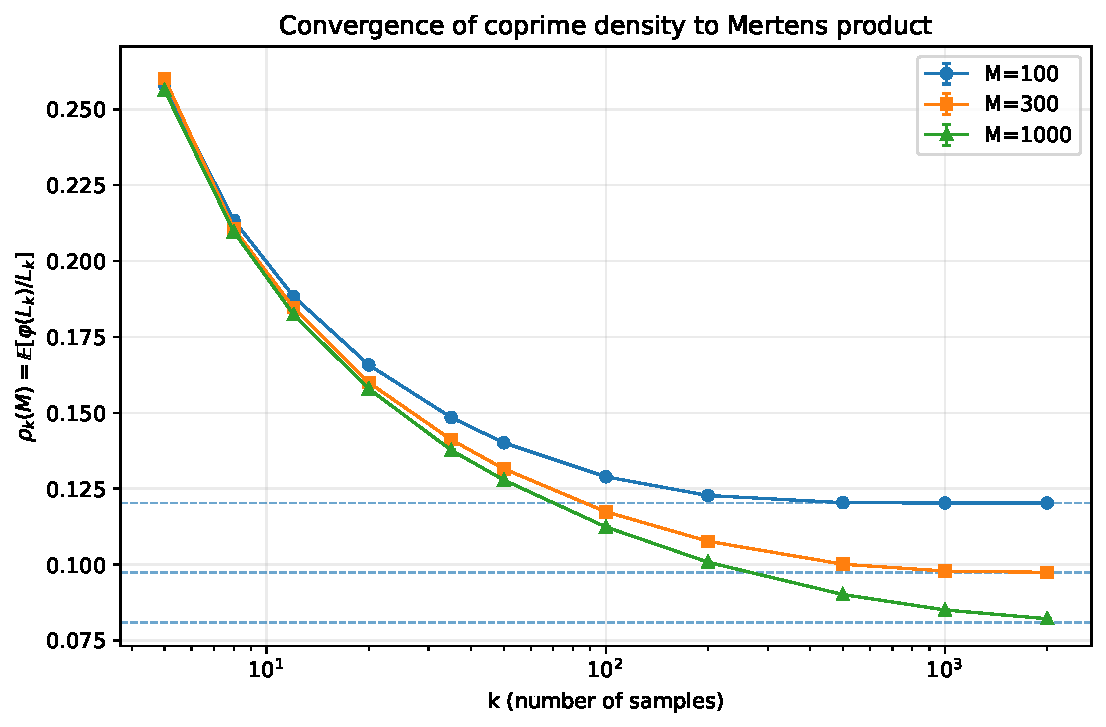
\includegraphics[width=0.85\linewidth]{fig1_convergence.pdf}
\caption{Monte Carlo estimates of $\rho_k(M)$ for $M \in \{100, 300, 1000\}$, based on $N = 2000$ independent replicates per point. Error bars show $\pm 1$ standard error of the sample mean. Dashed lines indicate the exact Mertens product $P_M$.}
\label{fig:convergence}
\end{figure}

\begin{table}[!htbp]
\centering
\caption{Comparison of Monte Carlo estimates of $\rho_k(M) - P_M$ ($N = 2000$ samples per cell, standard error $\lesssim 10^{-3}$) against the first-order prediction $P_M\, \Sigma_k(M)$ computed exactly. The ratio column demonstrates convergence to unity as $k$ grows, consistent with Theorem~\ref{thm:limit-rate}.}
\label{tab:thm2}
\begin{tabular}{rrrrrrr}
\toprule
$M$ & $k$ & $\rho_k(M)$ (MC) & $P_M$ (exact) & gap obs. & gap pred.\ (exact) & ratio \\
\midrule
100 & 50 & 0.14023 & 0.12032 & 0.01991 & 0.01855 & 1.073 \\
100 & 200 & 0.12280 & 0.12032 & 0.00248 & 0.00248 & 1.000 \\
300 & 100 & 0.11740 & 0.09746 & 0.01994 & 0.01826 & 1.092 \\
300 & 500 & 0.10013 & 0.09746 & 0.00267 & 0.00264 & 1.011 \\
1000 & 500 & 0.09025 & 0.08097 & 0.00929 & 0.00876 & 1.060 \\
1000 & 2000 & 0.08220 & 0.08097 & 0.00124 & 0.00122 & 1.016 \\
1000 & 5000 & 0.08102 & 0.08097 & 0.00006 & 0.00006 & 1.000 \\
3000 & 5000 & 0.07131 & 0.06997 & 0.00135 & 0.00133 & 1.015 \\
\bottomrule
\end{tabular}
\end{table}

\emph{Theorem~\ref{thm:sharp-fixed-M} (sharp form at fixed $M$).} Table~\ref{tab:sharp-fixed} exhibits $R_k(M)/\Sigma_k(M)$ for $M \in \{20, 30\}$ and $k \in \{20, 40, 80, 160\}$ alongside the theoretical upper bound $(q^{**}/q^{*})^k$ from Theorem~\ref{thm:sharp-fixed-M} (ignoring the $(M-1)e^{\Lambda(M)}$ prefactor). The observed ratio decays exponentially, in fact substantially faster than the bound requires: at $M=20$, the ratio falls from $4.5 \times 10^{-2}$ at $k=20$ to $1.2 \times 10^{-5}$ at $k=160$, while the bound predicts decay by factor $(17/18)^{140} \approx 3 \times 10^{-4}$.

\begin{table}[!htbp]
\centering
\caption{Observed ratio $R_k(M)/\Sigma_k(M)$ versus theoretical rate $(q^{**}(M)/q^{*}(M))^k$ from Theorem~\ref{thm:sharp-fixed-M}. The bound is not sharp but captures the exponential decay. For $M \geq 11$, $q^{**}/q^{*} = (M-3)/(M-2)$.}
\label{tab:sharp-fixed}
\small
\begin{tabular}{rrrr}
\toprule
$M$ & $k$ & $R_k/\Sigma_k$ (obs.) & $(q^{**}/q^*)^k$ (rate) \\
\midrule
20 & 20 & $4.52 \times 10^{-2}$ & $3.19 \times 10^{-1}$ \\
20 & 40 & $1.22 \times 10^{-2}$ & $1.02 \times 10^{-1}$ \\
20 & 80 & $1.15 \times 10^{-3}$ & $1.03 \times 10^{-2}$ \\
20 & 160 & $1.18 \times 10^{-5}$ & $1.07 \times 10^{-4}$ \\
\midrule
30 & 20 & $6.30 \times 10^{-2}$ & $4.83 \times 10^{-1}$ \\
30 & 40 & $2.27 \times 10^{-2}$ & $2.34 \times 10^{-1}$ \\
30 & 80 & $4.30 \times 10^{-3}$ & $5.45 \times 10^{-2}$ \\
30 & 160 & $2.20 \times 10^{-4}$ & $2.97 \times 10^{-3}$ \\
\bottomrule
\end{tabular}
\end{table}

\emph{Theorem~\ref{thm:joint-sharp}.} Figure~\ref{fig:joint} plots $\ln M \cdot \Sigma_{\lfloor cM \rfloor}(M)$ (computed exactly) at $M \in \{10^3, 10^4, 10^5, 10^6\}$ against $A(c)$; Table~\ref{tab:joint} extends to $M = 10^7$ across 15 values of $c \in [0.05, 15]$. The relative error $(\ln M \cdot \Sigma_{\lfloor cM \rfloor}(M) - A(c))/A(c)$ at $M = 10^7$ ranges from approximately $10.7\%$ at $c = 0.05$ down to $2.1\%$ at $c = 15$, decreasing monotonically in $c$; these residuals are consistent with the expected $O(1/\ln M)$ correction arising from the Meissel--Mertens constant in~\eqref{eq:mertens-strip}. Linear extrapolation of the sequence $\{\ln M \cdot \Sigma_{\lfloor cM \rfloor}(M)\}_M$ in the variable $1/\ln M$ (fitted over $M \in \{10^4, 10^5, 10^6, 10^7\}$) agrees with $A(c)$ to within approximately $0.5\%$ for $c \in [0.1, 5]$ and to within $1.5\%$ across the full tested range $c \in [0.05, 15]$.

\begin{figure}[!htbp]
\centering
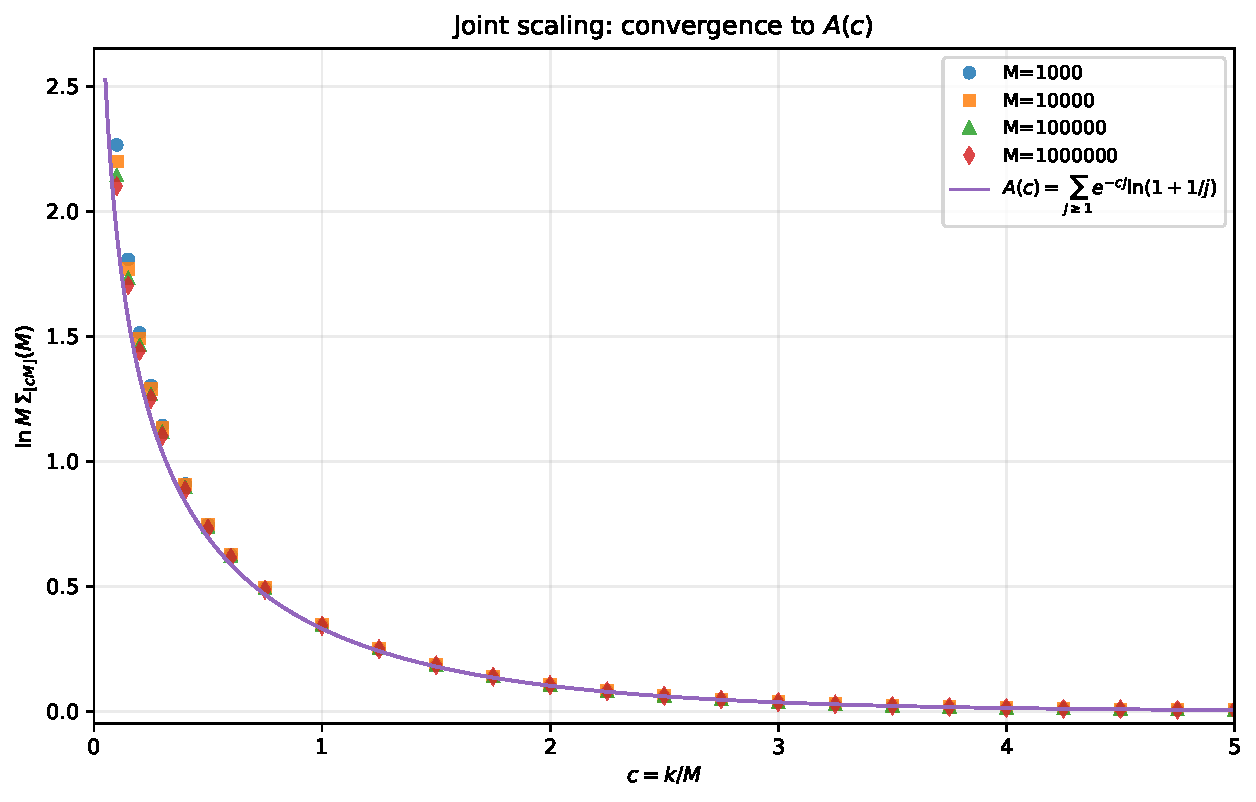
\includegraphics[width=0.85\linewidth]{fig2_joint_scaling.pdf}
\caption{Joint scaling regime $k = \lfloor cM \rfloor$. Points show $\ln M \cdot \Sigma_{\lfloor cM \rfloor}(M)$, computed exactly (no Monte Carlo) at $M \in \{10^3, 10^4, 10^5, 10^6\}$. Solid curve: $A(c) = \sum_{j \geq 1} e^{-cj} \ln(1 + 1/j)$, computed to $j_{\max} = 200$.}
\label{fig:joint}
\end{figure}

\begin{table}[!htbp]
\centering
\caption{$\ln M \cdot \Sigma_{\lfloor cM \rfloor}(M)$ versus $A(c)$ at $M$ up to $10^7$. All values computed exactly; no Monte Carlo. Residuals decay as expected from the $O(1/\ln M)$ Mertens-constant correction; see text.}
\label{tab:joint}
\small
\begin{tabular}{rrrrrr}
\toprule
$c$ & $A(c)$ & $M = 10^4$ & $M = 10^5$ & $M = 10^6$ & $M = 10^7$ \\
\midrule
0.05 & 2.5267 & 3.0277 & 2.9231 & 2.8498 & 2.7982 \\
0.10 & 1.9095 & 2.1999 & 2.1428 & 2.1009 & 2.0714 \\
0.15 & 1.5688 & 1.7704 & 1.7324 & 1.7033 & 1.6831 \\
0.25 & 1.1687 & 1.2886 & 1.2671 & 1.2498 & 1.2380 \\
0.50 & 0.6954 & 0.7470 & 0.7382 & 0.7307 & 0.7258 \\
0.75 & 0.4665 & 0.4950 & 0.4903 & 0.4861 & 0.4835 \\
1.00 & 0.3301 & 0.3476 & 0.3448 & 0.3422 & 0.3406 \\
1.25 & 0.2406 & 0.2522 & 0.2504 & 0.2486 & 0.2476 \\
1.50 & 0.1787 & 0.1867 & 0.1855 & 0.1843 & 0.1836 \\
2.00 & 0.1020 & 0.1061 & 0.1056 & 0.1049 & 0.1045 \\
3.00 & 0.0356 & 0.0368 & 0.0367 & 0.0365 & 0.0364 \\
5.00 & 0.00469 & 0.00485 & 0.00483 & 0.00480 & 0.00479 \\
7.50 & 0.000384 & 0.000396 & 0.000395 & 0.000393 & 0.000392 \\
10.00 & 0.0000315 & 0.0000325 & 0.0000324 & 0.0000322 & 0.0000321 \\
15.00 & 0.00000021 & 0.00000022 & 0.00000022 & 0.00000021 & 0.00000021 \\
\bottomrule
\end{tabular}
\end{table}

\section{Discussion and Open Problems}\label{sec:discussion}

\emph{Uniform vs.\ non-uniform rates.} Theorem~\ref{thm:sharp-fixed-M} gives an exponential rate at fixed $M$, but the rate $q^{**}(M)/q^{*}(M) = (M-3)/(M-2) \to 1$ degenerates as $M \to \infty$, so the bound does not yield the sharp joint-scaling result of Theorem~\ref{thm:joint-sharp}. The joint regime therefore requires a genuinely different mechanism (the geometric-mean bound Lemma~\ref{lem:geom-mean}).

\emph{Second-order fluctuations.} A natural next question is the scale and distributional shape of the fluctuations of $\ln(\varphi(L_k)/L_k)$ about its mean in the same joint regime: the variance asymptotic and an associated central limit theorem. These are developed in separate work in preparation.

\emph{General distributions.} Theorem~\ref{thm:identity} generalises verbatim to any distribution on $\{2, \ldots, M\}$, with $\beta_T(M)$ replaced by the probability of being coprime to $\prod_{p \in T} p$. Theorem~\ref{thm:limit-rate} generalises similarly. The joint scaling~\eqref{eq:sigma-limit} depends on the distribution of $m_p$-values, which is distribution-dependent.

\emph{Applications to non-uniform sampling diagnostics.} For distributions close to uniform, the function $A(c)$ is robust, but substantial departures from uniformity deform it in a distribution-specific way. Empirical estimates of $A(c)$ could therefore serve as a statistical test of uniformity for random integer generators over bounded ranges; a systematic development is left to future work.

\section{Conclusion}\label{sec:conclusion}

We have introduced the expected coprime density $\rho_k(M) = \EE[\varphi(L_k)/L_k]$ of the LCM of random integers in the regime of fixed support and growing sample size, and proved four theorems and one proposition. Theorem~\ref{thm:identity} establishes an exact finite-sum identity over subsets of $\PM$. Theorem~\ref{thm:limit-rate} shows $\rho_k(M) \to P_M$ at fixed $M$ with explicit rate. Theorem~\ref{thm:sharp-fixed-M} sharpens this to a full asymptotic equivalence at fixed $M$, with explicit geometric rate controlled by the ratio $q^{**}(M)/q^*(M)$ of the second-largest to largest single-prime coprime densities. Theorem~\ref{thm:joint-sharp} establishes the sharp joint-scaling equivalence $\ln M \cdot (\rho_{\lfloor cM \rfloor}(M) - P_M)/P_M \to A(c) := \sum_{j \geq 1} e^{-cj} \ln(1 + 1/j)$. The key new ingredient for Theorem~\ref{thm:joint-sharp} is the geometric-mean bound $\beta_T^k \leq \prod_{p \in T} q_p^{k/|T|}$ (Lemma~\ref{lem:geom-mean}), which permits control of the multi-prime corrections uniformly in the size of the subset. Proposition~\ref{prop:A-asymptotics} gives the $c \to 0^+$ and $c \to \infty$ asymptotics of $A$. Numerical computation up to $M = 10^7$ illustrates Theorem~\ref{thm:joint-sharp}. The regime studied here is complementary to the classical fixed-$k$ random-LCM literature; the exact subset identity (Theorem~\ref{thm:identity}) may be of independent use in related problems involving multiplicative functions of random LCMs.

\paragraph{Data and code availability.}
Source code, random seeds, and raw numerical output for all figures and tables are openly available at \url{https://github.com/Wakid90/coprime-density-lcm}.

\begin{thebibliography}{99}

\bibitem{AlsmeyerKabluchkoMarynych2019}
G.~Alsmeyer, Z.~Kabluchko, A.~Marynych, \emph{Limit theorems for the least common multiple of a random set of integers}, Trans.\ Amer.\ Math.\ Soc.\ 372 (2019), 4585--4603.

\bibitem{BostanMarynychRaschel2019}
A.~Bostan, A.~Marynych, K.~Raschel, \emph{On the least common multiple of several random integers}, J.\ Number Theory 204 (2019), 113--133.

\bibitem{BuraczewskiIksanovMarynych2022}
D.~Buraczewski, A.~Iksanov, A.~Marynych, \emph{Central limit theorem for the least common multiple of a uniformly sampled $m$-tuple of integers}, J.\ Number Theory 233 (2022), 301--336.

\bibitem{Cesaro1885}
E.~Ces\`aro, \emph{\'Etude moyenne du plus grand commun diviseur de deux nombres}, Ann.\ Mat.\ Pura Appl.\ 13 (1885), 235--250.

\bibitem{CilleruleoRueSarkaZumalacarregui2014}
J.~Cilleruelo, J.~Ru\'e, P.~\v{S}arka, A.~Zumalac\'arregui, \emph{The least common multiple of random sets of positive integers}, J.\ Number Theory 144 (2014), 92--104.

\bibitem{FernandezFernandez2021}
J.~L.~Fern\'andez, P.~Fern\'andez, \emph{Divisibility properties of random samples of integers}, Rev.\ Real Acad.\ Cienc.\ Exactas F\'is.\ Nat., Ser.\ A Mat.\ 115 (2021), article 26.

\bibitem{HilberdinkToth2016}
T.~Hilberdink, L.~T\'oth, \emph{On the average value of the least common multiple of $k$ positive integers}, J.\ Number Theory 169 (2016), 327--341.

\bibitem{IksanovMarynychRaschel2022}
A.~Iksanov, A.~Marynych, K.~Raschel, \emph{Asymptotics of arithmetic functions of GCD and LCM of random integers in hyperbolic regions}, Results Math.\ 77 (2022), article 165.

\bibitem{KabluchkoMarynychRaschel2023}
Z.~Kabluchko, A.~Marynych, K.~Raschel, \emph{Multivariate multiplicative functions of uniform random vectors in large integer domains}, Results Math.\ 78 (2023), article 201.

\bibitem{Lichtman2021}
J.~D.~Lichtman, \emph{Mertens' prime product formula, dissected}, Integers 21A (2021), article A17.

\bibitem{Ramanujan1919}
S.~Ramanujan, \emph{A proof of Bertrand's postulate}, J.\ Indian Math.\ Soc.\ 11 (1919), 181--182.

\bibitem{RosserSchoenfeld1962}
J.~B.~Rosser, L.~Schoenfeld, \emph{Approximate formulas for some functions of prime numbers}, Illinois J.\ Math.\ 6 (1962), 64--94.

\bibitem{Sanna2021}
C.~Sanna, \emph{On the least common multiple of random $q$-integers}, Res.\ Number Theory 7 (2021), article 16.

\bibitem{Tenenbaum2015}
G.~Tenenbaum, \emph{Introduction to Analytic and Probabilistic Number Theory}, 3rd ed., Graduate Studies in Mathematics 163, Amer.\ Math.\ Soc., 2015.

\end{thebibliography}

\end{document}
